%\documentclass[a4paper,11pt]{scrreprt}
%\documentclass[a4paper,15pt]{scrbook}
\documentclass[a4paper,12pt]{scrartcl}
%\documentclass[a4paper,13pt]{scrreprt}

\usepackage[T1]{fontenc}
\usepackage[utf8]{inputenc}
%\usepackage[latin9]{inputenc}
\usepackage{scrpage2}
\usepackage{titleref}
\usepackage[ngerman]{babel}
\usepackage{multicol}
\usepackage{lmodern}  
\usepackage{tabularx} 
\usepackage{graphicx}
\usepackage{blindtext}
\usepackage{microtype}
\usepackage{color}
\usepackage{colortbl}
\usepackage{framed} %umramen eines Bereiches
%\usepackage[left=25mm,right=25mm,top=25mm,bottom=25mm]{geometry} % Standard
%\usepackage[left=20mm,right=20mm,top=25mm,bottom=30mm]{geometry}
%\usepackage[singlespacing]{setspace}
\usepackage[onehalfspacing]{setspace}
%\usepackage[doublespacing]{setspace}%
\usepackage{verbatim}
\usepackage{listings}
%\usepackage[svgnames]{xcolor}
\usepackage{xcolor} 
\usepackage{setspace}
\usepackage{amsthm}
\usepackage{float}
\usepackage{pdfpages}
\usepackage{mdwlist}
\usepackage{prettyref}
\usepackage{multicol}
\usepackage[section]{minted}	
\usepackage{hyperref}

%%%%%% Beschriftung
\newcommand{\changefont}[3]{
\fontfamily{#1}\fontseries{#2}\fontshape{#3}\selectfont}


%\include{./color}
%\include{./environment}
%\input{./minted}
%\input{./listings}	
	
\begin{document}
%-------------------------------------
% Titelseite 
\thispagestyle{empty}
\begin{center}
	
\includegraphics[scale=.5]{./fau}\\
	\vspace*{2cm}
	\Large
	\textbf{Informatik}\\
	\textbf{Marketing Fallstudien}\\
	\vspace*{2cm}
	\Huge
	\textbf{Hausarbeit}\\
	\vspace*{0.5cm}
	\large
	über das Thema\\
	\vspace*{1cm}
	\textbf{Neue Gefahren durch neue Apps und Foren wie YouNow und Snapchat}\\
	\vspace*{2cm}
	
	\vfill
	\normalsize
	\newcolumntype{x}[1]{>{\raggedleft\arraybackslash\hspace{0pt}}p{#1}}
	\begin{tabular}{x{6cm}p{7.5cm}}
		\rule{0mm}{5ex}\textbf{Autor:} & Johannes Pfann \newline johannes.pfann@fau.de \\
		\rule{0mm}{5ex}\textbf{Autor:} & Johannes Stadlinger \newline johannes.stadlinger@fau.de \\
		\rule{0mm}{5ex}\textbf{Abgabedatum:} & \today \\
	\end{tabular} 
\end{center}
\pagebreak

%-------------------------------------

%-------------------------------------
% Verzeichnisse  
\tableofcontents % Inhaltsverzeichnis
\pagebreak
%\listoffigures % Abbildungsverzeichnis 
%\listoftables % Tabellenverzeichnis 
%-------------------------------------

%-------------------------------------
% Textkörper
%%%%%%%%%%%%%%%%%%%%%[Einleitung]
\section{Zusammenfassung}
Das Thema soziale Netzwerke wurde in den letzten Jahren immer populärer. In den letzten 5 Jahren hat sich die Anzahl mehr als verdoppelt. Vor allem durch Mobile Anwendungen hat sich die Benutzung dieser soziale Netzwerke dramatisch verändert. Problematisch ist dabei, das Jugendliche sich der Konsequenz dieser Veränderung nicht bewusst sind.
Die folgende Hausarbeit beschäftigt sich mit Gefahren durch die Apps und Foren wie YouNow und Snapchat im Rahmen der Veranstaltung Marketing Fallstudie. Ziel dieser Arbeit ist ein grundsätzliches Verständnis der Anwendungen YouNow und Snap-Chat zu beschreiben um dann die Gefahren durch Pädophilie und Datenschutzrecht zu erläutern.
 


\section{Einleitung}
Das Thema \emph{soziale Netzwerke} wurde in den letzten Jahren immer
popul\"arer. Wie man in Abbildung~\ref{fig:overall} sieht, waren es im Jahr
2010 lediglich knapp eine Milliarde Nutzer weltweit, die sich in solchen
Netzwerken angemeldet hatten. Die Zahl stieg stetig an. Innerhalb von f\"unf
Jahren (2015) hat sich diese Anzahl mehr als verdoppelt auf $2,14$ Milliarden
Nutzer. Das stetige Wachstum wird auch f\"ur die Zukunft prognostiziert.
\begin{figure}[ht]
	\centering
	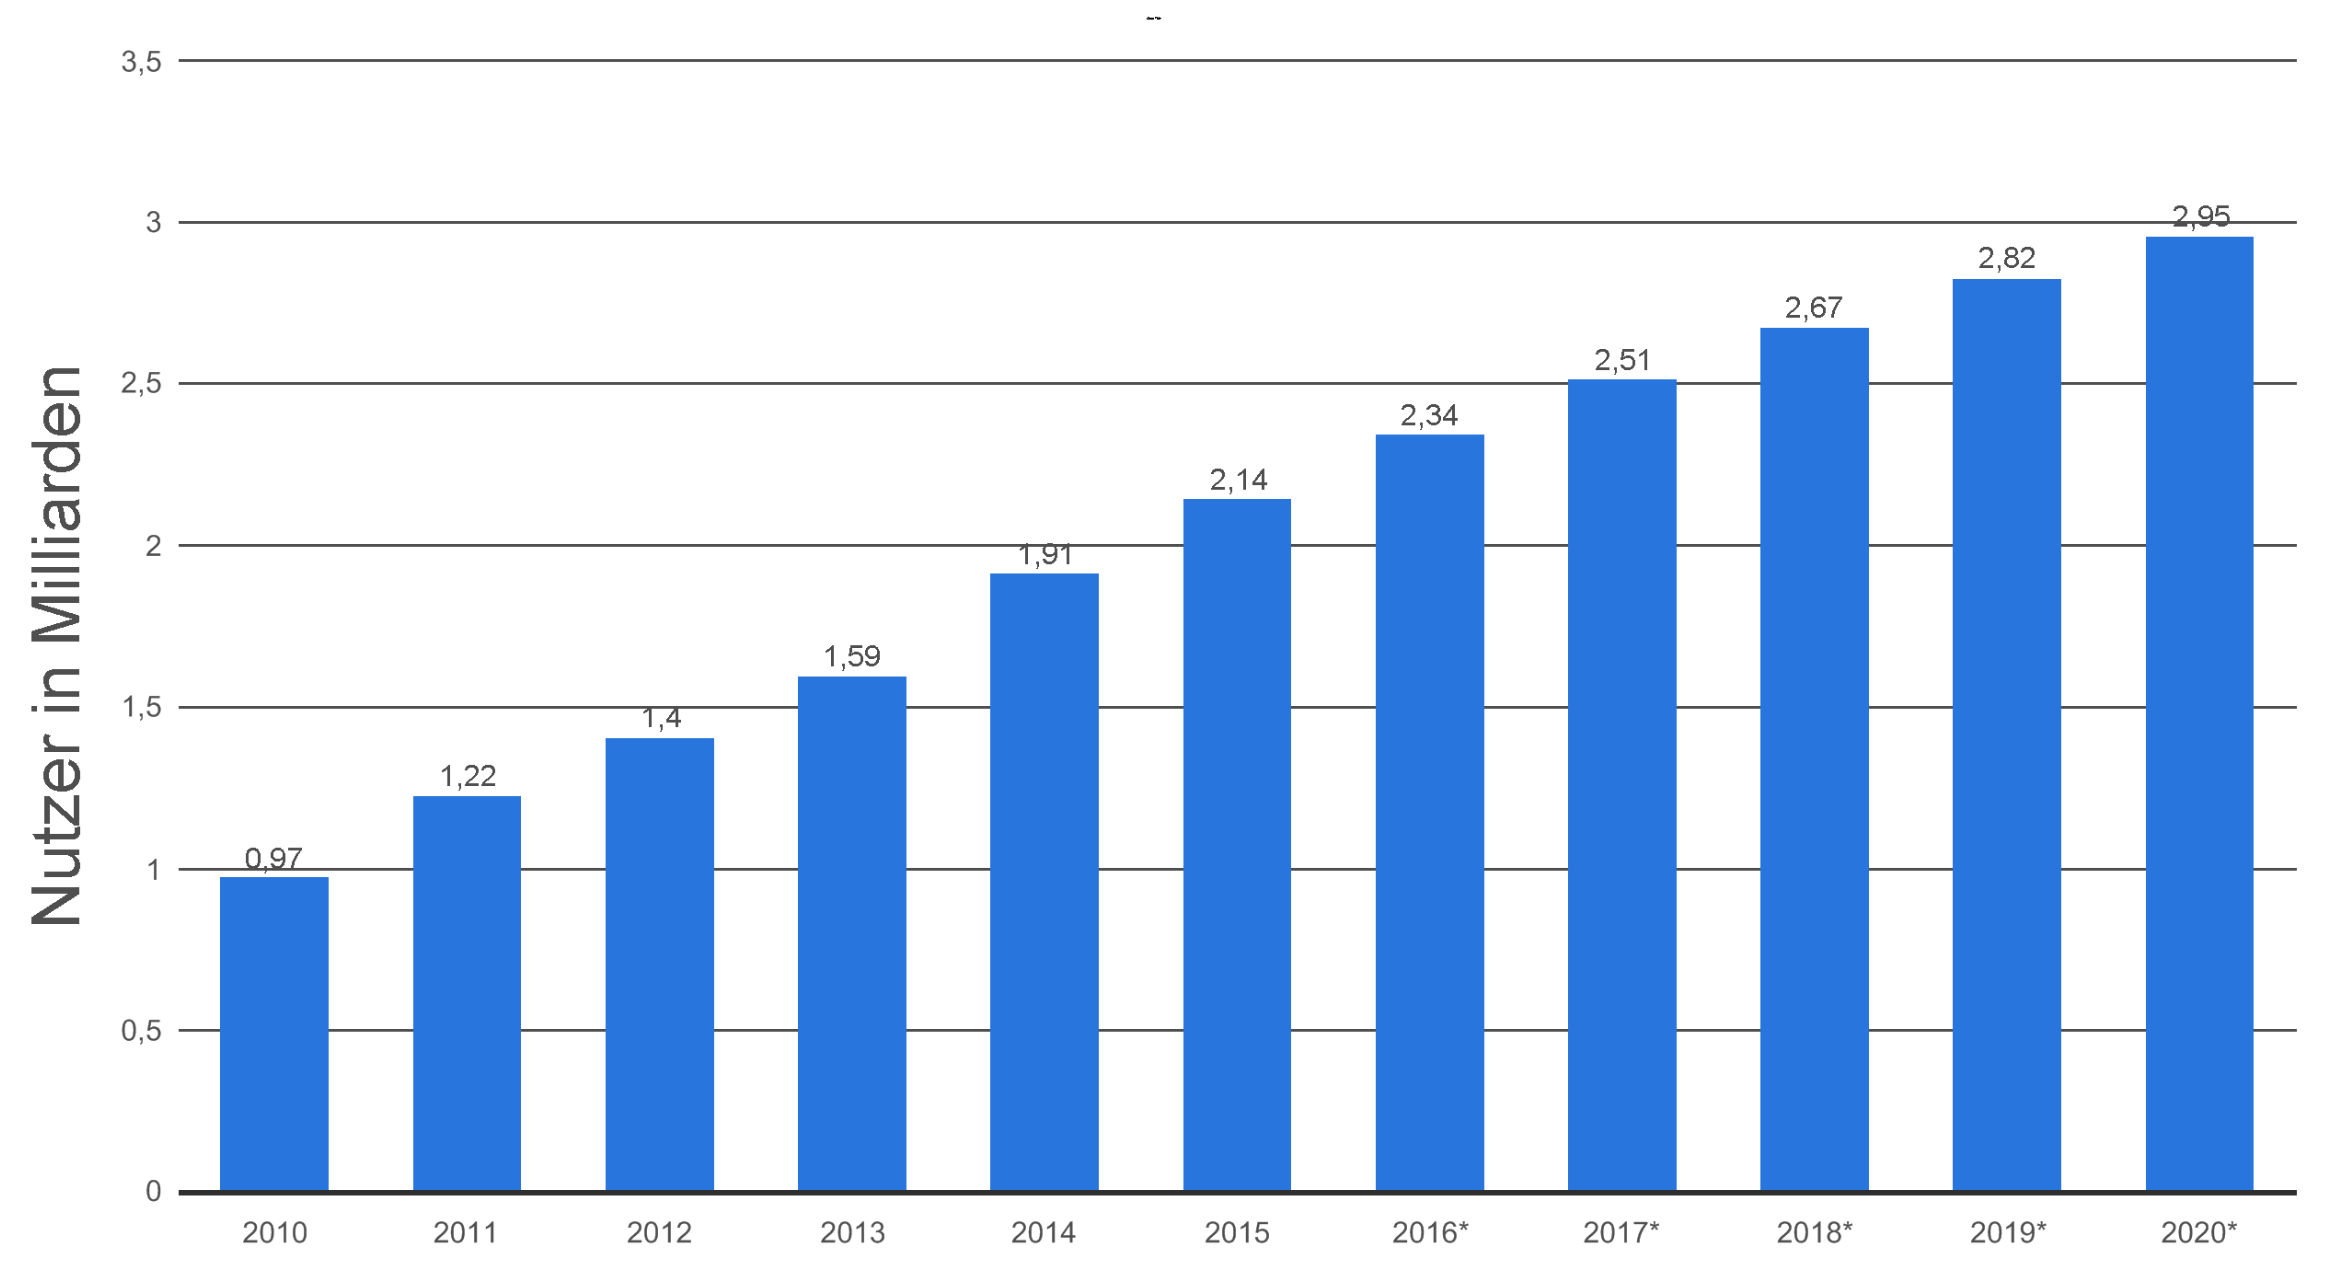
\includegraphics[scale=0.6]{resources/einf_02.png}
	\caption{Anzahl der Nutzer sozialer Netzwerke weltweit in den Jahren 2010
	bis 2015 sowie eine Prognose bis 2020 (in Milliarden)~\cite{statista-allg}.}
	\label{fig:overall}
\end{figure}

//hier noch etwas text. Uebergang von allg. zu Jugendlichen. evtl noch mehr statistiks

YouNow\footnote{\url{https://www.younow.com}} und
SnapChat\footnote{\url{https://www.snapchat.com}} sind zwei aufstrebende,
neuere Anwendungen in diesem Bereich und vor allem bei Kindern und Jugendlichen
sehr beliebt~\cite{statista-snapchat, vaterlaus2016snapchat}. Im Rahmen dieser Arbeit werden beide
etwas n\"aher betrachtet und auf m\"ogliche Gefahren in Bezug auf P\"adophilie
untersucht.



\section{YouNow}
\subsection{Beschreibung}
YouNow ist eine kostenlose Live-Videostreaming-Plattform, die als App auf dem Smartphone oder als Desktop-Anwendung verfügbar ist. Nutzer können nach einer Anmeldung mit der Kamera ihres Smartphones, Laptop oder Tablets Live-Streams von sich aufnehmen und für andere Nutzer bereitstellen oder bei dessen Live-Streams zusehen. Neben der Möglichkeit des Live-Streams bietet die Plattform einen Chat an, sodass in einem Live-Stream alle Beteiligten miteinander kommunizieren können. Außerdem kann ein weiterer Nutzer sich an einem Video beteiligen. 

\paragraph{Anmeldung}
Nach Installation der App auf dem Smartphone oder dem Öffnen der Website mit dem Browser kann man sich mit Facebook, Gmail- oder Twitter-Account anmelden. Diese Anmeldung erfordert allerdings sämtliche Kontaktdaten und Email-Adressen des Kontoinhabers. Außerdem muss man versichern, das man nicht jünger als 13 Jahre alt ist.
Im nächsten Schritt wird man aufgefordert einen Namen anzugeben, mit dem man in Videos und Chats erkannt wird.

\paragraph{Kommunikation}
Während des Live-Streams ist gleichzeitig ein Chat aktiv, mit dem sich der Protagonist mit seinen Zuschauern unterhalten kann. Chatteilnehmer können sich Nachrichten, Sticker oder Icons zusenden. Neben den Chats, ermöglicht die App das Versenden von Posts zu einzelnen Personen. Diese erscheinen, ähnlich wie bei der Facebook-Chronik, auf einer Pinnwand der jeweiligen Person. Außerdem können sich YouNow-Nutzer private Nachrichten zusenden.


\paragraph{Geschenke und Währung}
Bei YouNow gibt es zwei verschiedene Währungen die jeweils für verschiedene Aktionen gedacht sind. Zum einen gibt es Münzen (Coints), die repräsentieren einen Wert eines Geschenkes. Mit einem Geschenk, kann ein Zuschauer auf sich aufmerksam machen bzw. den Stream eines anderen wertschätzen, indem er ein Geschenk für diesen versendet. Geschenke sind in diesem Fall kleine Bilder (Icons).
Coints haben keinen realen Gegenwert und müssen in YouNow verdient werden. Mit folgenden Aktionen können Coints verdient werden:

\begin{itemize}
	\item Veröffentlichen von Livestreams
	\item Aktive Teilnahme. Durch das Anschauen von Livestreams, Liken oder chatten kann man Münzen verdienen.
	\item Deine Freunde für eine Anmeldung bei YouNow werben. Für jede Anmeldung deiner Freunde über einen Facebook-Post, Tweet, E-Mail, Tumblr-Verlinkung oder Facebook-Einladung von dir erhältst Du Münzen. 
	\item Dich jeden Tag anmelden.
\end{itemize} 

Eine weitere Währung sind die sog. \textbf{bars}. Diese können nicht durch Aktionen erworben werden, sondern müssen gekauft werden. Die haben also einen realen Gegenwert. Mit diesen können dann Premiumgeschenke gekauft werden, mit denen man sich in einem Chat besonders auf sich aufmerksam machen kann. Premiumgeschenke könnten sein:

\begin{itemize}
	\item 50 Likes: Ein Geschenk, dass den Broadcaster hilft zu trenden
	\item Fanpost: Eine personalisierte Chat-Nachricht, die heraussticht 
	\item 50 Likes für den eigenen Stream: Hilft dem Broadcaster, mehr Aufmerksamkeit zu erlangen
	\item Chat-cool-down-bypass: Aufhebung der Begrenzung der eigenen Chatnachrichten in vollen, überlasteten Chats
	\item Bars: Um Partner unmittelbar zu unterstützen
\end{itemize}

\paragraph{Levelsystem}
YouNow führt außerdem ein Levelsystem ein. Dieses hat die Aufgabe den Nutzer dazu anzuregen mehr Aktionen auf YouNow zu tätigen. Der Anreiz um weitere Levels zu bekommen ist, dass der Nutzer dadurch Zugriff auf bessere und speziellere Geschenke erlangt um den Streamenden zu unterstützen. Außerdem steigt pro Level auch der Wert an Münzen, die dann auf die normalen Geschenke berechnet werden. 
Um ein höheres Level zu erreichen hat der Nutzer folgende Möglichkeiten.

\begin{itemize}
	\item je mehr Geschenke sie selbst erhalten
	\item je mehr Likes sie erhalten
	\item je größer ihr Publikum ist
	\item je mehr Live-Streams sie tätigen
	\item je mehr sie mit anderen Nutzern chatten
	\item je mehr Geschenke sie selbst vergeben
	\item je mehr Freunde sie zu YouNow einladen.
	\item und, wenn sie ihre Konten aus anderen Sozialen Netzwerken, wie z. B. YouTube, Facebook, Twitter mit ihrem YouNow-Konto verknüpfen.
\end{itemize}

\subsection{Datenschutz und Profil}
YouNow gibt in seinen Richtlinien vor, wie man sich verhalten soll. Zusätzlich gibt es die Möglichkeit in seinem Profil Angaben zu verbergen.

\paragraph{Personenbezogene Daten}
YouNow garantiert auf seiner Homepage, keine Daten zu veröffentlichen oder an Dritte weiterzugeben. Jedoch räumt YouNow ein, für Behörden auf Anfrage einer Strafverfolgung nachzukommen. Außerdem schreiben die Richtlinien vor, keine E-Mailadresse, Telefonnummern oder Wohnadressen anderer zu veröffentlichen. Bei Verstoß verspricht YouNow, dies mit einer temporären oder dauerhaften Sperrung zu ahnden.

\paragraph{Profil}
Für den erstellten Account besteht die Möglichkeit dessen Profil zu bearbeiten (siehe Abbildung~\ref{profil_einstellungen}). Einstellungen in dem Profil sind kein Zwang, denn auch ohne lassen sich alle Funktionen der Plattform nutzen. In den Einstellungen kann man sein Profil- und Hintergrundbild einstellen, einen Nickname und eine Kurzbeschreibung. Außerdem kann hier entschieden werden, ob der richtige Name oder der Nickname in Chats erscheinen soll und ob man seinen Standort preisgeben möchte.

\begin{figure}[ht!]
\centering
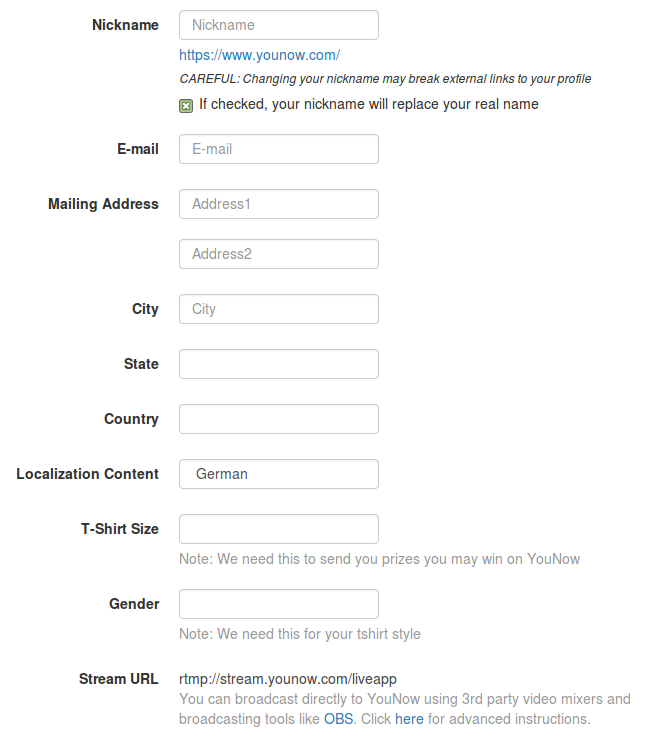
\includegraphics[width=0.7\textwidth]{./resources/younow_profile_settings}
\caption{YouNow-Profileinstellung. Freiwillige Angaben innerhalb des Profils.}
\label{profil_einstellungen}
\end{figure} 

\subsection{Kritik}
Die größte Problematik besteht darin, das Nutzer nur wenig darauf achten, wie sie mit den neuen Medien umgehen. Speziell bei YouNow ergeben sich folgende Problemstellungen, welche auf der Internetseite \cite{KS15} vorgestellt werden.

% \paragraph{Übertragung in Echtzeit}
% Da die Übertragung in Echtzeit geschieht, folgt daraus die Problematik, das nichts zurückgenommen werden kann. Schnell kann passieren das persönliche Daten preisgegeben werden oder Meinungen, die unbedacht geäußert werden. Außerdem können viel Informationen durch emotionale Reaktionen preisgegeben werden, wenn beispielsweise auf bestimmte Fragen ungewöhnlich reagiert wird. Diese sind dann für alle sichtbar und können im Nachhinein nicht revidiert werden.

\paragraph{Persönlichkeitsrecht}
Es besteht die Möglichkeit, das im Hintergrund Personen sich aufhalten, denen nicht bewusst ist, das sich gerade in einem Live-Stream sind. Das ist jedoch ein Verstoß gegen das Recht am eigenen Bild. Ein weiteres Problem stellt eine Zeit-Autorin dar. Viele interviewen oder filmen ihre kleineren Geschwister, die sich nicht bewusst sein können, welche Konsequenzen YouNow für sie haben (siehe \cite{ZEIT15}).
Außerdem wird im Hintergrund oft Musik gespielt. Dies kann als Urheberrechtsverletzung gewertet werden. Eine Studie zeigt, dass 37 \% aller Broadcasts aus Deutschland gegen das Urheberrecht verstoßen (siehe \cite{HFMNF15}).

\paragraph{Jugendschutz}
Obwohl YouNow in seinen Regeln und bei der Anmeldung deutlich macht, dass sich keine Jugendlichen unter 13 Jahren anmelden dürfen, kann dies nicht kontrolliert werden. Es gibt Moderatoren, die bei Missachtung des Mindestalters diejenigen sperren, was aber nur schwer zu kontrollieren ist, wenn keine Angaben darüber gemacht werden. Außerdem kann aufgrund der Masse an Live-Streams nicht gewährleistet werden, dass alle anstößigen Inhalte auch zügig von den Moderatoren entfernt werden. Ein speziell für das Thema herausgebrachtes Schreiben (siehe \cite{YTD15}) von YouNow macht deutlich, das dies durchaus ein Problem für den Dienstanbieter darstellt. 

\paragraph{Ungewollten Kontaktaufnahme}
Da man als Moderator eines Live-Streams sein Publikum nicht sieht, kann man auch nicht wissen, wer unter einem Pseudonym chattet und welche Intention die jeweilige Person damit verfolgt. Außerdem kann man auch ohne Anmeldung einen Live-Streams beobachten.





\section{Snapchat}
\subsection{Beschreibung}
Snapchat ist eine kostenlose Smartphone Anwendung f\"ur Android und iOS, die es
seinen Nutzern erm\"oglicht Bild- sowie Videonachrichten zu versenden. Die App
wurde im September 2011 initial released und ist mittlerweile in $20$ Sprachen
\"ubersetzt. Im Gegensatz zu YouNow gibt es f\"ur Snapchat keine
Desktopvariante.

Eine Besonderheit gegen\"uber anderen Anwendungen ist, dass die Medieninhalte
nur f\"ur begrenzte Zeit, d.h. mindestens eine und maximal $10$ Sekunden
f\"ur den/die Empf\"anger sichtbar sind. Nach diesem Zeitraum l\"oschen sich
laut Anbieter die Dateien von selbst beim Client. Mittlerweile ist es jedoch
m\"oglich die Inhalte mehrfach anzusehen. Zudem kann ein Nutzer eine sogenannte
,,Snapchat-Geschichte'' anlegen, welche $24$ Stunden sichtbar und mit
bestimmten Freunden oder der gesamten Community teilbar ist.

\paragraph{Anmeldung}
Bevor man die Anwendung auf seinen Smartphone installieren kann, muss man
Snapchat umfangreiche Rechte zugestehen. Abbildung~\ref{fig:sc_perms} zeigt
examplarisch die Rechteanfordungen unter Android.
\begin{figure}[ht]
	\centering
	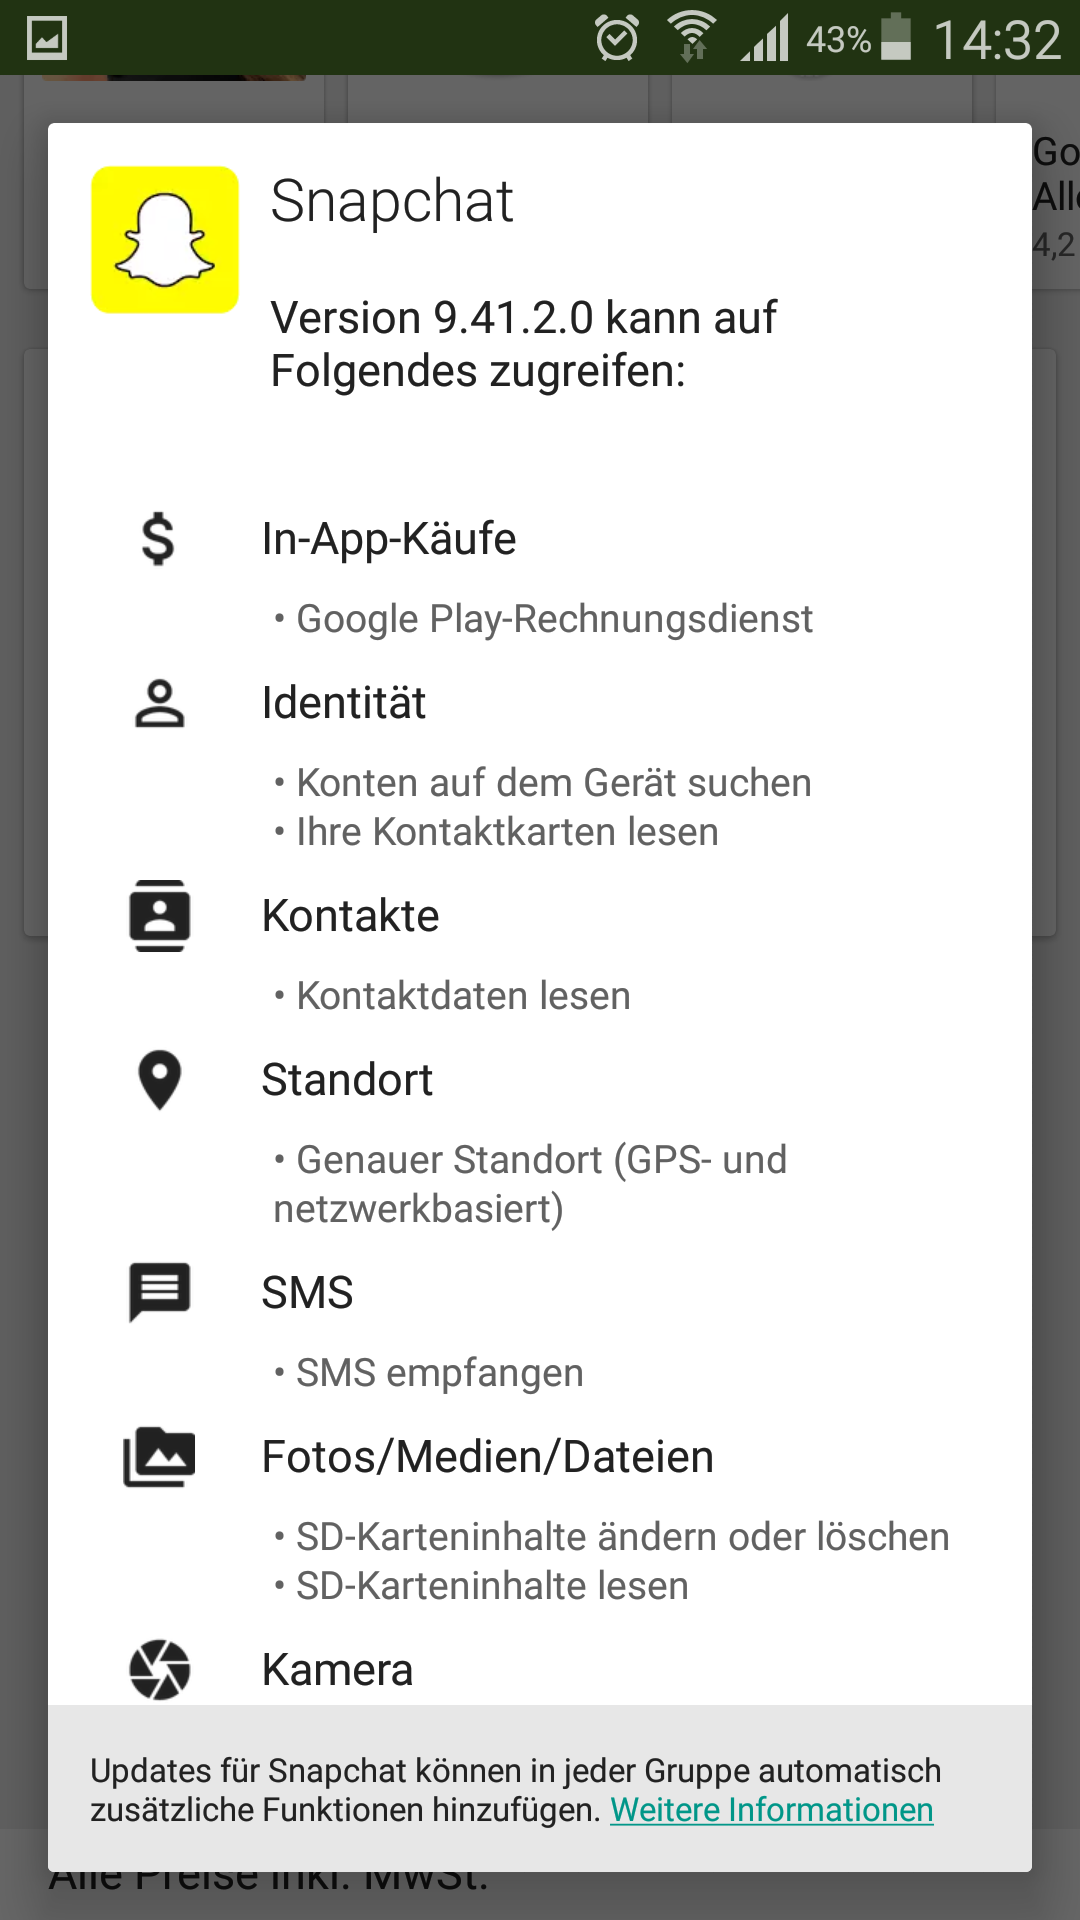
\includegraphics[width=0.4\linewidth]{resources/sc_perms_1.png}
	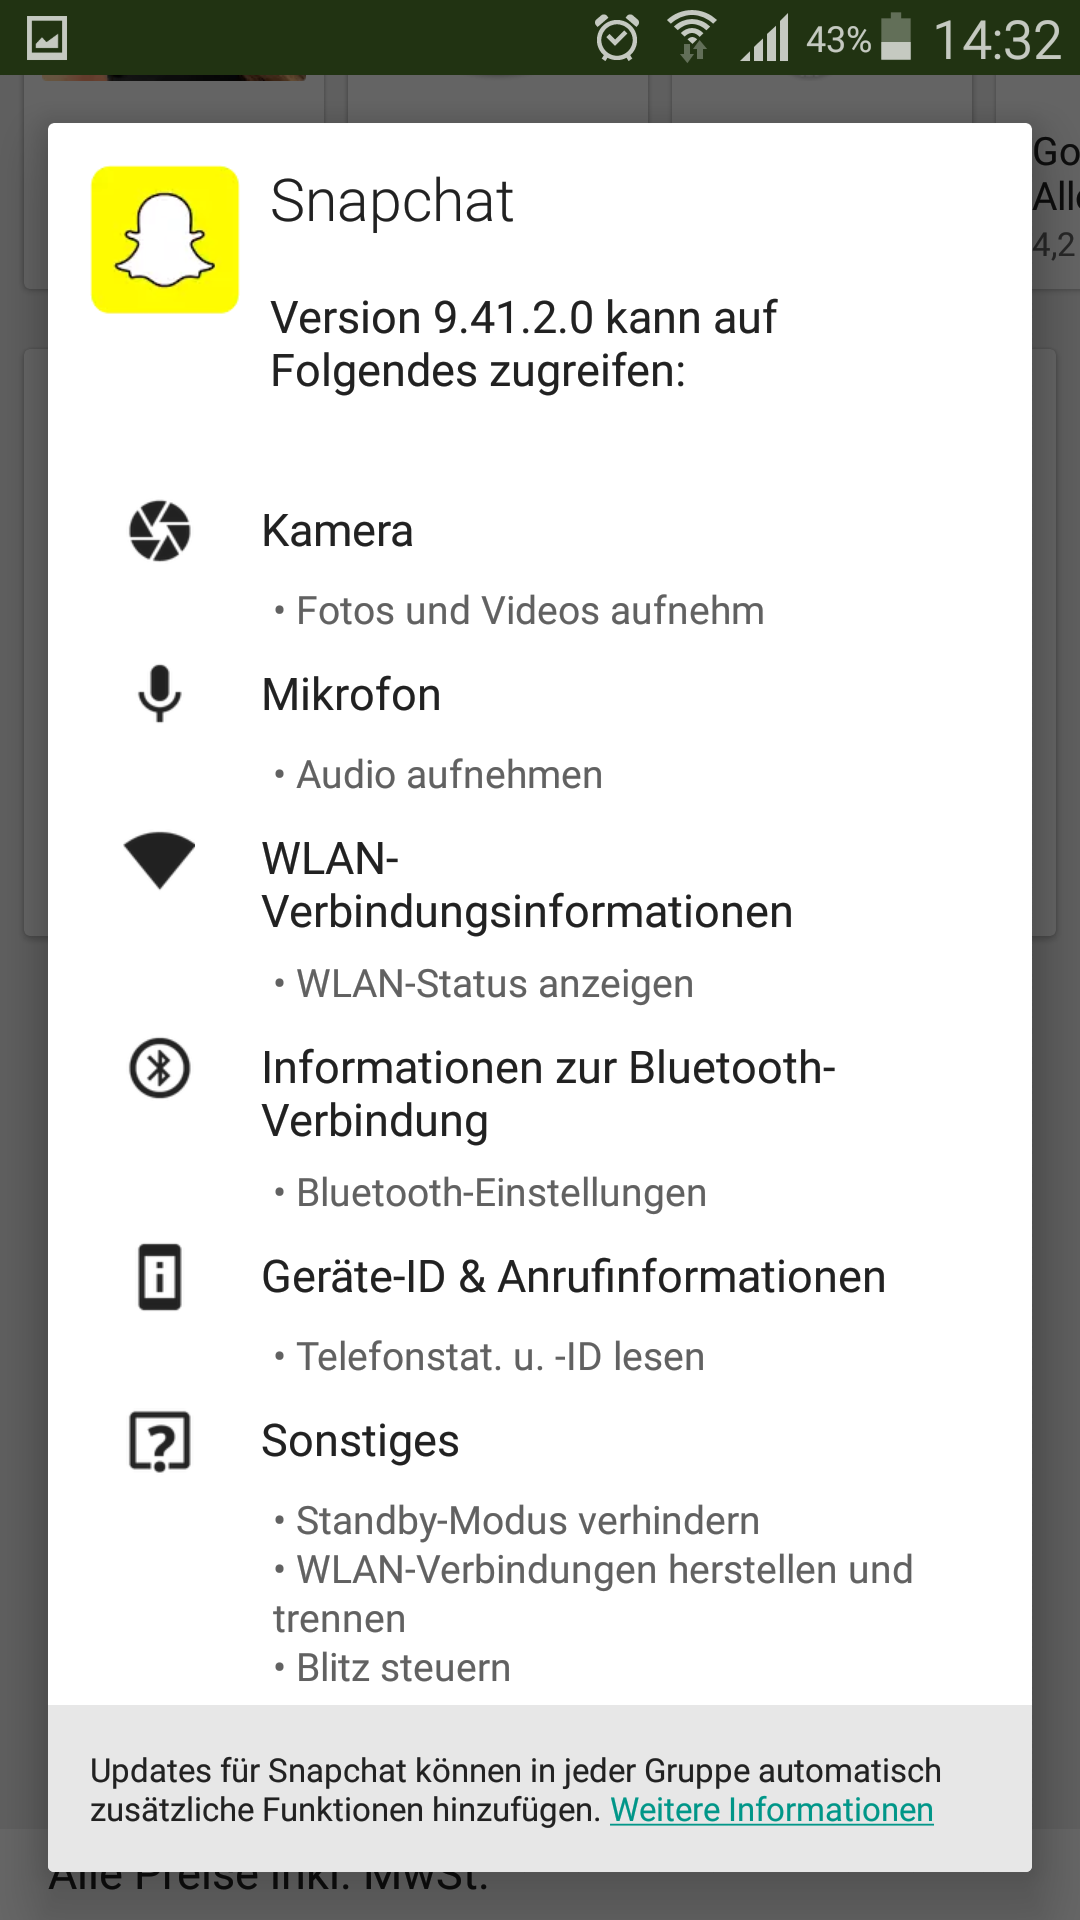
\includegraphics[width=0.4\linewidth]{resources/sc_perms_2.png}
	\label{fig:sc_perms}
	\caption{\"Ubersicht der Rechteanforderung von Snapchat auf einem Android
	Smartphone.}
\end{figure}
Unter anderem muss der App das Auslesen s\"amtlicher Kontakt- sowie
Standortdaten des Ger\"ats gew\"ahrleistet werden. Auch der Zugriff auf
Fotos, Videos, Medien sowie Kamera und Mikrofon muss freigegeben werden.

Ist die App auf dem Ger\"at installiert kann man sich als Nutzer anmelden.
Hierf\"ur ist eine Email-Adresse, ein Nutzername, das Geburtsdatum, sowie ein
Passwort erforderlich. Eine Kontrolle des Alters wird vom Anbieter nicht
durchgefuehrt.

\paragraph{Funktionsweise und Kommunikation}
In diesem Abschnitt m\"ochten wir noch etwas genauer auf die Funktionsweise und
Kommunikation von Snapchat eingehen.

Um \"uberhaupt Inhalte zu Versenden braucht der neu angemeldete Nutzer Personen
mit denen er kommunizieren kann. Diese kann er \"uber folgende M\"oglichkeiten
hinzuf\"ugen:
\begin{itemize}
	\item Nutzernamen: Eingabe konkreter Nutzer.
	\item Aus Kontakten: Kontaktliste des Smartphones nach Personen mit
	Snapchat durchsuchen lassen.
	\item Snapcode: Vergleichbar mit QR-Codes.
	\item In der N\"ahe: Nutzer, die im gleichen Wlan-Netz sind.
\end{itemize}

Jetzt hat der Nutzer die M\"oglichkeit sogenannte \emph{Snaps} d.h. Fotos oder
Videos aufzunehmen bzw. aus der Gallerie zu entnehmen und diese mit Text,
Filtern, etc. zu bearbeiten. Anschliessend kann er diese an seine Freunde
schicken. Wie eingangs erw\"ahnt, kann er nun auch festlegen, wie lange das
Medium auf dem Ger\"at des Empf\"angers sichtbar bleibt (eine bis max. zehn
Sekunden). Nach diesem Zeitraum wird das Datum vom Endger\"at gel\"oscht. Zudem
hat er die M\"oglichkeit das Medium seiner eigenen \emph{Geschichte} (engl.:
\emph{story}) hinzuzuf\"ugen damit es $24$ Stunden sichtbar bleibt. Von dort
aus kann er seine Snaps mit Freunden oder mit der ganzen Community teilen. Die
Inhalte k\"onnen dann von allen Beteiligten gespeichert werden.

Neben der M\"oglichkeit seinen Partnern Text-, Bild- und Snapnachrichten zu
schicken, bietet Snapchat auch einen Videochat an. Hier kann man sich in
Echtzeit mit seinem Gegen\"uber mit Hilfe seiner Smartphonekamera unterhalten.

\subsection{Datenschutz und -nutzung}
Auf der offiziellen Internetseite von Snapchat~\cite{snap_site} propagiert das
Unternehmen den hohen Stellenwert von Datenschutz. Jedoch werden bei der
Nutzung von Snapchat und seinen Services Daten von Nutzern gesammelt. Um eine
hohe Transparenz zu gew\"ahrleisten, beschreibt das Unternehmen, welche Daten
zu welchen Zweck erhoben werden. Das Unternehmen unterscheidet in folgende Gruppen:
\begin{enumerate}
	\item Vom Nutzer freiwillig zur Verf\"ugung gestellte Daten
	\item Daten, die durch die Nutzung der Services anfallen
	\item Daten durch Dritte
\end{enumerate}
Im folgenden gehen wir auf die \emph{Datenschutzbestimmungen} etwas
n\"aher ein.

\paragraph{Vom Nutzer freiwillig gestellte Daten}
Um Snapchat nutzen zu k\"onnen braucht man einen Nutzeraccount f\"ur dessen
Erstellung man Informationen wie Name, Email-Adresse, Passwort, Alter und ggf.
Rufnummer angeben muss. Sein Profil kann man zudem noch weiter bearbeiten,
indem man ein Profilbild oder andere hilfreiche Informationen von sich
preisgibt. Diese Daten werden vom Unternehmen gespeichert. Kommerzielle Dienste
innerhalb der App ben\"otigen ggf.  Kreditkartennummern oder andere
Zahlungsinformationen. Deine gesendeten Bilder und Videos k\"onnen zum einen
vom Empf\"anger gespeichert werden (z.B. durch Screenshot) und werden ebenfalls
auch von Snapchat gespeichert.

\paragraph{Daten, durch das Benutzen von Services}
Die Anwendung sammelt eine Vielzahl von Daten, die durch das Benutzen der
Services anfallen. Das beinhaltet \emph{Nutzungsdaten} wie z.B. wie man mit
anderen Personen kommuniziert oder wie der User bestimmte Services nutzt.
Au{\ss}erdem werden die Inhalte jeder Kommunikation sowie ger\"atespezifische
Daten wie Telefonbuch, Kamera, Gallery und Standortdaten gespeichert.

\paragraph{Daten von Dritten}
Snapchat kann Daten erfassen, die von anderen Nutzern \"uber einen bestimmten
preisgegeben werden. Zum Beispiel, wenn ein bestimmter Nutzer A im Telefonbuch
eines Nutzers B aufgef\"uhrt wird, kann Snapchat diese Kontaktdaten mit den
Daten von Nutzer A zusammenf\"uhren.

\paragraph{Nutzung von Daten}
Das Unternehmen verabeitet die Daten demhingegehend, dass sie zum einen mit
ihren Nutzern kommunizieren und die eigentliche Anwendung weiterentwickeln
k\"onnen. Zum anderen wird aus den Daten personalisierte Werbung verbessert,
angepasst und ausgeliefert.

\paragraph{Weitergabe von Daten}
Die Daten von Nutzern kann von Snapchat auf folgende Weise weitergegeben werden:
\begin{itemize}
	\item \emph{An andere Snapchat-User}: Daten zu einer Person wie Name und
		Alter als auch weitere Daten, die der Nutzer freiwillig abgibt,
		k\"onnen an andere Nutzer weitergegeben werden, um bestimmte Personen
		schneller zu finden.
	\item \emph{An die \"Offentlichkeit}: Profilbilder, Snapcodes, und Medien,
		die ein Nutzer an \"offentliche Channels sendet.
	\item \emph{An Dritte}: Snapchat finanziert sich durch Werbung.
		Dementsprechend werden die personenbezogenen Daten an Drittanbieter aus
		der Werbebranche weitergegeben. Auch beh\"alt sich Snapchat das Recht,
		Daten aus rechtlichen Gr\"unden bei Missbrauch oder anderen
		Verst\"o{\ss}en offenzulegen.
	\item \emph{Aggregierte und anonymisierte Date}: Diese Daten werden
		ebenfalls an Werbeunternehmen weitergegeben.
\end{itemize}

\subsection{Community-Richtlinien}
Snapchat besitzt Community-Richtlinien und Standards~\cite{sc_richtlinien} um
einen sicheren Umgang mit der Anwendung zu gew\"ahrleisten. Werden diese nicht
eingehalten, kann es zu Sperrung bzw. L\"oschung des Accounts f\"uhren. Die
wichtigsten Ans\"atze der Richtlinien werden im Folgenden kurz
zusammengetragen.

\paragraph{Allgemeines}
Es wird darauf hingewiesen, dass die Nutzer sich klar sein sollten, was sie
\"uber Snapchat teilen. Insbesondere wird nochmals explizit darauf hingewiesen,
dass der Gegen\"uber die M\"oglichkeit besitzt, gesendete Daten
\emph{abzufotographieren} oder andersweitig zu \emph{vervielf\"altigen}. Zudem
betont das Unternehmen, dass die Inhalte \emph{legal} sein sollten.

\paragraph{Verbotene Inhalte}
Snapchat weist explizit darauf hin, dass jede Art von \emph{Pornographie} in
ihrem Netzwerk verboten ist. Das beinhaltet ein Verbot zur Verbreitung von
pornographischen und nicht jugendfreien Inhalt, angedeutete sexuelle Handlung,
sowie Nacktheit in Verbindung mit sexuellen Handlungen.

Jugendliche sollen besonders gesch\"utzt werden. Deswegen untersagt Snapchat
das Versenden von \emph{Nacktdarstellungen oder sexuell aufreizende Inhalte von
Minderj\"ahrigen}.

Zudem weist das Unterehmen darauf hin, dass es verboten ist, Bilder oder Videos
von Dritten ohne deren Zustimmung zu versenden. Auch das Drohen bzw. Mobben
anderer Nutzer wird untersagt.

\subsection{Kritik}
Genauso wie bei YouNow, besteht auch bei Snapchat das gr\"o{\ss}te Problem
darin, dass die Nutzer zu leichtsinnig mit ihren privaten Daten umgehen. Auch
hier gibt es verschiedene Initiativen, die den User aufkl\"aren und die
schwerwiegendsten Kritiken offenbaren~\cite{sc_risiken}. 

\paragraph{Haltbarkeit von Daten}
Snapchat gibt in seinen ABGs an, dass die Daten, die ein User verschickt, nur
f\"ur einen bestimmten Zeitraum auf dem Endger\"at des Empf\"angers vorhanden
und anschlie{\ss}end gel\"oscht werden. In der Praxis sieht das leider etwas
anders aus: Die Dateien werden lediglich mit einer anderen Endung versehen,
damit Gallerie-Apps diese nicht mehr finden und anzeigen k\"onnen. Somit
bleiben die Inhalte auf dem Ger\"at vorhanden und k\"onnen mit etwas Aufwand
wiederhergestellt werden.

Was man auch noch bedenken muss, wenn man private Bilder via Snapchat
versendet, mit dem Hintergedanken, dass sie nur kurz f\"ur den Empf\"anger
sichtbar sind, ist, dass der Empf\"anger immer noch die M\"oglichkeit besitzt,
die Inhalte per Screenshot oder mit einem zus\"atzlichen Aufnahmeger\"at
sichern kann~\cite{sc_risiken}.

\paragraph{Datenschutz}
Ein weiterer Kritikpunkt ist Snapchats Umgang mit den Daten seiner User. Wie
bereits erw\"ahnt sammelt das Unternehmen eine Reihe personenbezogener Daten
und der Nutzer willigt automatisch den Datennutzungsbestimmungen (siehe oben)
und damit verbundene Weiterverarbeitung und -gabe zu. Medieninhalte wie Bilder
und Videos werden bis zum Abruf vom Empf\"anger auf den Servern, welche in den
Vereinigten Staaten stehen, gespeichert. Innerhalb dieses Zeitraums hat
Snapchat vollen und freien Zugriff auf die Bilddateien seiner
User~\cite{sc_risiken}.


\section{Angriffsvektoren}

Im nachfolgenden Abschnitt werden mögliche Wege zweier Angriffsziele aufgezeigt, die Personen bei jugendliche Nutzer anwenden können. Zunächst wird ein Graph eingeführt, der diese Angriffsszenarien verbildlicht. Danach wird die Umsetzung dieser Schritte mit den jeweiligen Apps erklärt. 

\begin{figure}[h!]
\centering
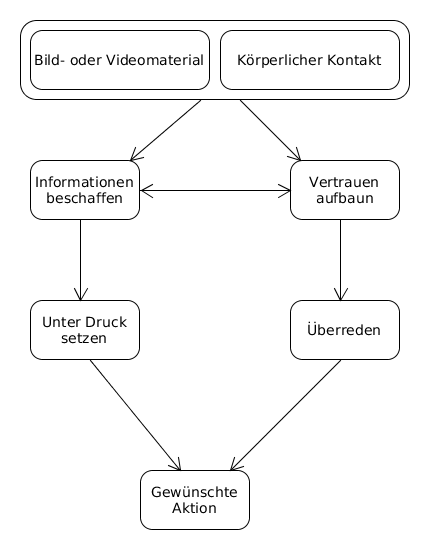
\includegraphics[width=0.5\textwidth]{./resources/angriffsvektoren}
\caption{Einfache Angriffswege}
\label{vektoren_overview}
\end{figure} 

%
In Abbildung \ref{vektoren_overview} werden zwei mögliche Ziele und deren Umsetzungsschritte vereinfacht verbildlicht. Dabei werden nicht alle möglichen Schritte und deren Kombinationen abgehandelt. Das Schaubild soll lediglich zwei einfache Szenarien behandeln um jeweils zwei mögliche Ziele zu erreichen. Als erstes Ziel wird die Beschaffung von Bild- oder Videomaterial von der jugendliche Person definiert.
Das zweite Ziel ist der körperliche Kontakt, der eine Person zu der oder dem Jugendlichen erreichen möchte.

\subsection{Informationen beschaffen um damit Druck auszuüben.}

Die Idee bei diesem Weg ist, so viel Informationen zu beschaffen, mit dem der oder die Jugendliche unter Druck gesetzt werden kann. Ein Druckmittel könnte ein Geheimnis von den Eltern oder unangenehme Informationen von den Jugendlichen sein. Mit diesen Druckmittel kann dann das Opfer für Handlungen gezwungen werden. Diese Praktiken nennt man Social Engineering. Dabei versucht man durch zwischenmenschliche Beeinflussung Personen dazu bringen bestimmte Verhaltensweisen hervorzurufen, wie beispielsweise persönliche Informationen preiszugeben.

\paragraph{Bei YouNow} kann jeder, auch ohne eine Anmeldung die Videos von Jugendlichen ansehen, ohne dass die betreffende Person etwas davon mitbekommt. Hier wäre es möglich über einen längeren Zeitraum belastende  Informationen zu suchen. Denkbar wäre auch gezielte Fragen zu stellen, mit denen man weitere Schritte unternehmen könnte. Dazu müsste man sich allerdings anmelden. 

\paragraph{Bei Snapchat} ...

\subsection{Vertrauen aufbauen um die betreffende Person zu überreden.}
Für diesen Schritt muss sich der Jugendliche über einen gewissen Zeitraum auf die Person einlassen. Denkbar wäre im Vorfeld eine Informationsbeschaffung um gezielter zu manipulieren oder das Vertrauen für die Beschaffung zu nutzen. 

\paragraph{Bei YouNow}, wie bei allen anderen Internetdiensten, ist es nicht möglich sicherzustellen, dass sich hinter einer Person auch diese verbirgt. Man kann ohne weiteres sich einen Account erstellen.  Für die Kontaktaufnahme ist der Chat neben dem Stream zur Verfügung. Außerdem gibt es noch die Möglichkeit dem Jugendlichen persönlich zu schreiben. 

\paragraph{Bei Snapchat} ...
\subsection{Empfehlung für den Umgang mit YouNow}
Um sicher YouNow zu nutzen, können einfache Regeln beachtet werden. 

\paragraph{Wenig Profilinformationen}
Da es nicht erforderlich ist, sein Profil mit allen Informationen zu befüllen, sollte nur das nötigste angegeben werden. Wohnort und Kontaktdaten möglichst nicht ausfüllen. Außerdem sollte niemals der eigene Name als Nickname verwendet werden.


\paragraph{Informationen ausblenden}
Unter den Profileinstellungen kann man die Option \textit{hide my city} anklicken. Dadurch wird der Wohnort verborgen. (siehe Abbildung \ref{privats_einstellung})

\begin{figure}[!ht]
\centering
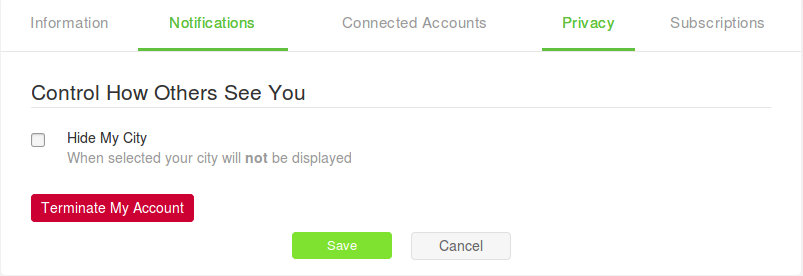
\includegraphics[width=0.6\textwidth]{./resources/younow_hide_my_city}
\caption{Einstellungen für die Privatsphäre}
\label{privats_einstellung}
\end{figure} 

\paragraph{Nutzer melden/blockieren}
Sind Personen aufdringlich oder beleidigend, kann man diese blockieren, sodass sie dann keine Möglichkeit mehr haben, Kontakt aufzunehmen. Allerdings gilt das nur für angemeldete Nutzer. Der Live-Stream ist weiterhin für jedermann zugänglich.
Möchte man einen anderen Nutzer melden, weil er gegen eines der YouNow Regeln verstoßen hat, kann man dies über die Melde-Funktion machen. Eine weitere Option besteht darin, direkt Kontakt mit einem Moderator aufzunehmen. Hierbei gibt es ein Kontaktformular. Hier müssen Angaben wie der Grund, eine Beschreibung und ggf. ein Screenshots angeben.

\paragraph{Antworten vorbereiten}
Während eines Live-Streams werden die Streamenden oft nach dem Alter, Wohnort bzw. Adresse oder anderen persönlichen Fragen gefragt. Hier empfiehlt es sich, vorab darüber nachzudenken, wie man darauf antworten könnte. So kann bei der Frage nach dem Wohnort bzw. Adresse eine sehr ungenaue Antwort wie: \glqq Ich komme aus Bayern\grqq geantwortet werden. Und bei weiteren Nachfragen könnte man bestimmt antworten: \glqq Genauer möchte ich nicht darauf eingehen\grqq .
Weiter kann man sich die eigene häusliche Umgebung für den Live-Stream gut ansehen und persönliche Dinge in dem Zimmer entfernen bevor man den Stream startet. 

\subsection{Skandale}
Nachfolgend werden einzelne Beiträge aus Pressemitteilungen aufgelistet die einen Einblick auf die Schattenseiten des YouNow-Protals zeigen sollen. Das dies durchaus ein Problem für den Betreiber YouNow darstellt, zeigt der Artikel von YouNow, in dem dieser verstärkt Moderatoren für die Einhaltung der Regeln einstellen wolle und er sich verstärkt um Minderjährige Nutzer kümmern möchte (siehe \cite{YTD15}).

\paragraph{Weiblicher Fan wird vor der Kamera zum Ausziehen überredet}
Ein sehr harter Vorfall zeigt, wie ein Nutzer einen anderen weiblichen Fan befragt, ob sie mit ihm Geschlechtsverkehr haben möchte. Als sie dieses bejaht, geht er einen Schritt weiter und fragt diese, ob sie auch Oralverkehr mache. Nach einer weiteren Bejahung fordert er sie dazu auf sich vor der Kamera auszuziehen. Dabei gibt er vor, alle anderen aus dem Chat geblockt zu haben, damit keiner etwas sieht. Nachdem der weibliche Fan auch noch den BH auszieht, gibt er zu, das jeder in seinem Live-Stream zugesehen habe (siehe \cite{MD10}).

\paragraph{Stern-Online warnt vor YouNow}
In einem Artikel im Stern (siehe \cite{STERN15}) wird an die Eltern appelliert mehr in Erfahrung zu bringen, welche Medien ihre Kinder nutzen. Diese sollten das Gespräch suchen und vor den Gefahren aufklären. Zu sehen ist in dem Artikel ein weiblicher Nutzer mit einem Zettel auf dem steht: \glqq Bei 200 Likes könnt ihr mich im BH sehen\grqq .

\paragraph{Rechtsanwälte klären auf}
Die Rechtsanwaltskanzlei WILDE BEUGER SOMECKE warnt vor den Rechtlichen Fallstricken des YouNow-Portals (siehe \cite{WBS15}). Hier wird darauf aufmerksam gemacht, dass das Filmen von Unterricht nicht legal sei. Außerdem entstehen Urheberrechtsverletzungen, weil Nutzer im Hintergrund Musik laufen ließen. Ein Studie zeigte auf, das 37 \% aller Broadcasts aus Deutschland gegen das Urheberrecht. Weitere 12 \% gegen Persönlichkeitsrecht, 8 \% enthalten Beleidigungen oder zeigen Drogenkonsum von Minderjährigen (siehe \cite{HFMNF15}).



\pagebreak

%%%%%%%%%%%%%%%%%%%%%[Quellen]
\section{Quellen}
%%%%%%%%%%%%%%%%%%%%%%%%%%%%%%%%%%%%%%%%%%%%%%%%%%%%%%%%%%%%%%%%%%%%%%%%%%%%%%%
%
%  http://www.weinelt.de/latex/thebibliography.html
%  \bibitem[Markierung]{Kennung}Quelle
%  \cite[Spezifikation]{Kennung}
%  \cite{GARR05}) kann auf die Quelle zugegriffen werden
%
%%%%%%%%%%%%%%%%%%%%%%%%%%%%%%%%%%%%%%%%%%%%%%%%%%%%%%%%%%%%%%%%%%%%%%%%%%%%%%%

\begin{thebibliography}{12cm}

\bibitem[GOF95]{GOF95} Erich Gamma, Richard Helm, Ralph E. Johnson, John Vlissides: Entwurfsmuster. Elemente wiederverwendbarer objektorientierter Software. Addison-Wesley, München 2004, ISBN 3-8273-2199-9.

\bibitem[EIST06]{EIST06} Karl Eilebrecht, Gernot Starke: Patterns Kompakt: Entwurfsmuster für effektive Softwareentwicklung Spektrum Akademischer Verlag, 4 Auflage 2006, ISBN 3-8274-1443-1

\bibitem[IN15]{IN15} Michael Inden: Der Weg zum Java-Profi: Konzepte und Techniken für die professionelle Java-Entwicklung, dpunkt.verlag,Heidelberg 2015, ISBN 978-86490-203-1

   

\end{thebibliography}


\end{document}
